\documentclass[12pt]{suvresdpl}

\author{Bartosz Błyszcz; Aleksander Filek}
\tGroup{01}
\tField{Informatyka Techniczna}
\tFaculty{WIMiIP}
\date{10-05-2022}
\tIndex{PSI}
\title{Wykorzystanie biblioteki Pytorch do modelowania sieci FNN}
\secTitle{Zastosowanie biblioteki Pytorch w aplikacji Unity}


\begin{document}
    \simplefancypage    
    \headAndFootWithShort
    
    \RedefinePlainStyle
	\setcounter{tocdepth}{2}
	\tableofcontents

    \chapter{Projekt}
\section{wstęp}
Aplikacja została przygotowana na potrzeby przedmiotu \textit{''Podstawy Sztucznej Inteligencji''}. Do jej wykonania wykorzystano repozytorium \textbf{ArztSamuel/Applying\_EANNs}\cite{aeann_psi}. Zadanie polegało na zastosowaniu biblioteki Pytorch\cite{pytorch}, dla języka Python. Należało połączyć skrypt, napisany w języku python do obliczania aktualnej zmiany pozycji dla pojazdu na mapie za pomocą \textbf{Jednokierunkowej Sieci Neuronowej}(ang. \textit{Feedforward Neural Network (FNN)}), wraz z aplikacją Unity napisanej w języku C$\#$; Dodatkowo należało dołączyć ten skrypt do algorytmu genetycznego (\textbf{GA}). Połączenie GA i FNN służy do wytrenowania pojazdów autonomicznych, których celem jest przejechanie utworzonej trasy.  

\subsection{Feedforward Neural Network}
Jest to typ sieci neuronowej, która jest jednokierunkowa (od wejścia, do wyjścia). W takich sieciach nie ma możliwości przepływ informacji w drugą stronę.\cite{lnn}

\begin{figure}[H]
    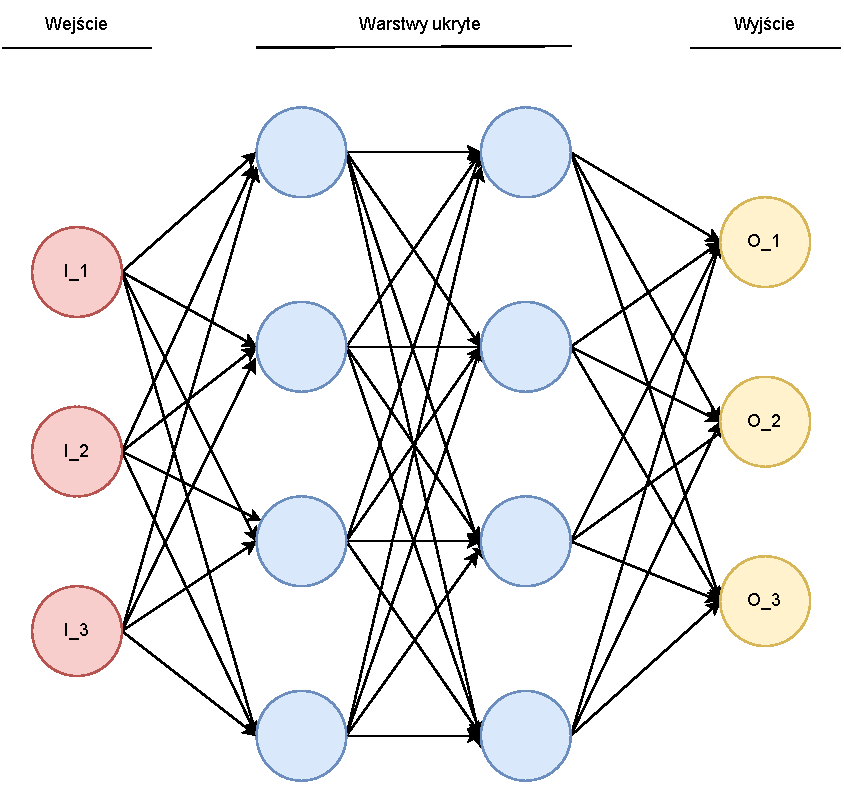
\includegraphics[width=\textwidth]{images/fnn.pdf}
    \caption{Schemat sieci neuronowej FNN}
    \label{fig:fnn}
\end{figure}

\subsection{Algorytm genetyczny}
Zdaniem algorytmu genetycznego jest znalezienie optymalnego rozwiązania w skończonej liczbie iteracji, bądź obejmującego minimalny optymalny wynik dopasowania. Algorytm polega na losowym utworzeniu populacji możliwych wyników, a następnie próbie ich dopasowania. Najlepiej dopasowane wyniki są wybierane, i przy zastosowanym w kodzie \textbf{wybieraniu elitarnym} zachowywane do następnej populacji. Następnie występuje krzyżowanie oraz mutacja wyników. Celem tych dwóch operacji jest wyłonienie potencjalnych najlepszych wyników. Po operacji mutowania wybierane są najlepsze rozwiązania z możliwym uwzględnieniem ''elitarnych'' wyników z pierwszej selekcji. Operacje się powtarza aż do znalezienia optymalnego rozwiązania, bądź przejściu maksymalnej ilości iteracji. Następnie jest zwracany ostatnie otrzymane rozwiązanie.

\begin{figure}[H]
    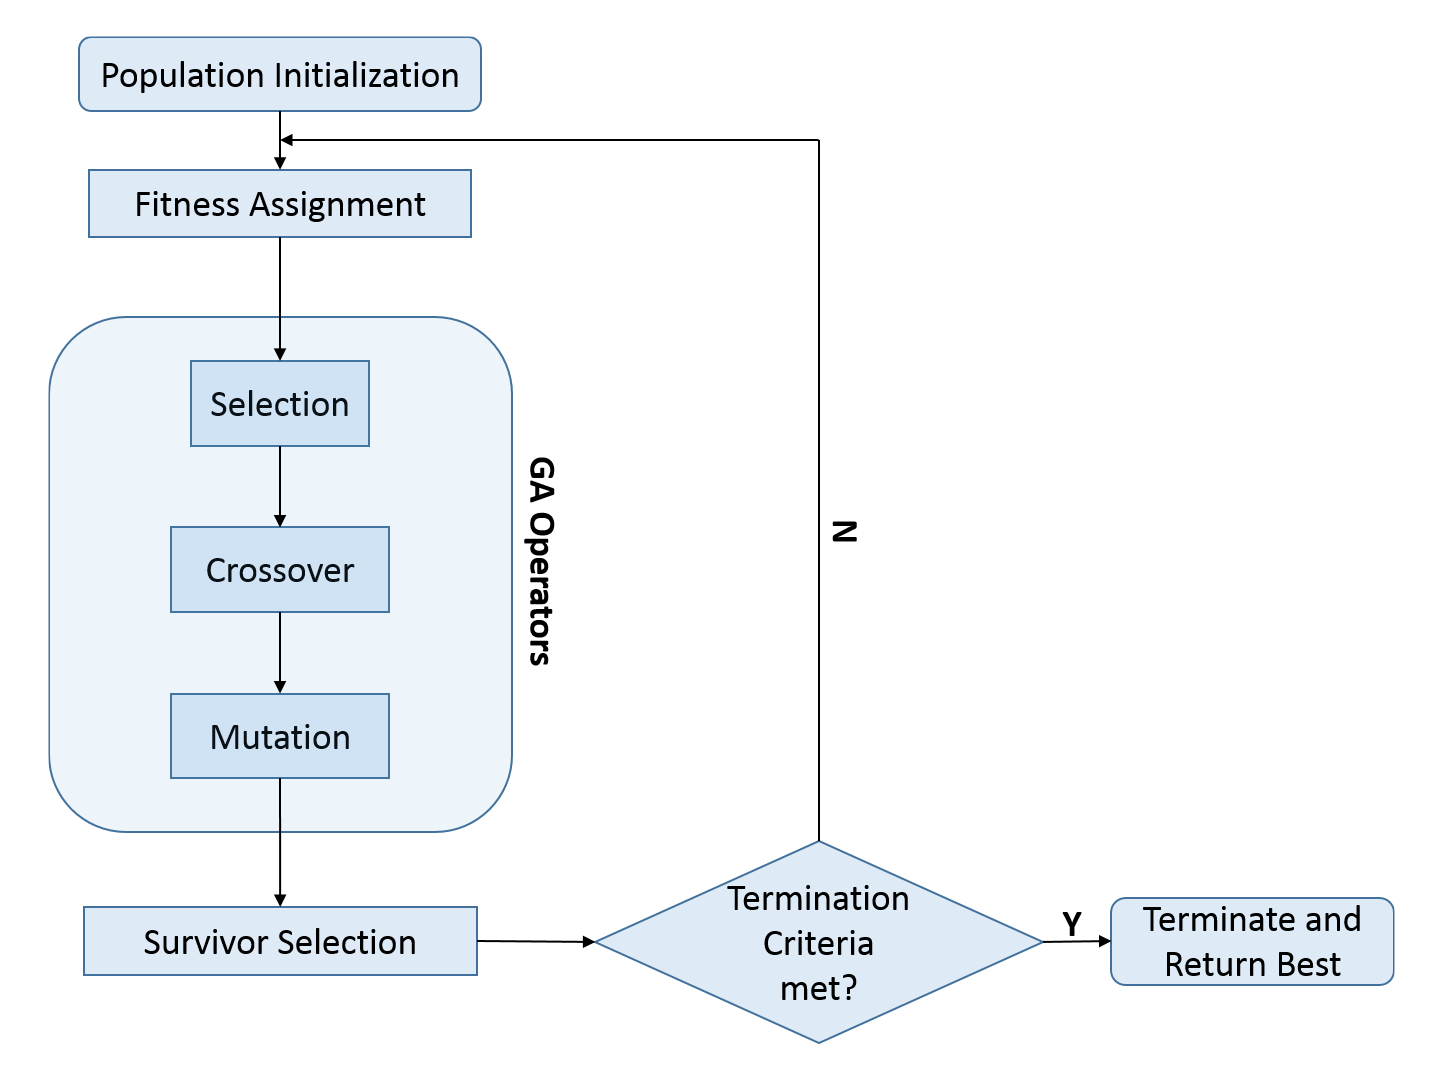
\includegraphics[width=\textwidth]{images/ga_schema.png}
    \label{fig:ga}
    \caption{Schemat algorytmu genetycznego\cite{ai}}
\end{figure}
    \printbibliography
\end{document}